\documentclass[titlepage,hidelinks,10pt]{article}
\usepackage[utf8]{inputenc}
\usepackage{parskip}
\usepackage[UKenglish]{babel}
\usepackage[headheight=15pt,margin=2cm]{geometry}
\usepackage{multicol}
\usepackage{multirow}
\usepackage[colorlinks=false]{hyperref}
\usepackage[super,square]{natbib}
\usepackage{float}
\usepackage[toc,page]{appendix}
\usepackage[table]{xcolor}
\usepackage{titling}
\usepackage{array}

\usepackage{color}
\usepackage{listings}
\usepackage{graphicx}
\graphicspath{ {img/} }
\usepackage{caption}
\usepackage{wrapfig}
\usepackage{lscape}
\usepackage{rotating}
\usepackage{epstopdf}
\usepackage{pifont}
\usepackage{gensymb}

\setlength{\parindent}{2em}

\date{January 2017}
\title{Augmented Reality Debugging System for Swarm Robotics \vspace{1cm}\\\Large{Initial Report}}
\author{Alistair Jewers}

\begin{document}

\maketitle

\tableofcontents
\newpage

\begin{multicols}{2}


\section{Project Overview and Aims}
Swarm Robotics is the name given to the nascent field of study focusing on the use of concepts derived from the study of social insects, such as ants or bees, to design and implement behavioural algorithms for multi-robot systems. These behaviours should allow a group of relatively simple robots to achieve a more complex, emergent behaviour, through cooperation\cite{SwarmRoboticsDefinition}. The broader area of study, without the robotics focus, is referred to as Swarm Intelligence (SI), and is described by Dorigo \& Birattari as the \textit{``discipline that deals with natural and artificial systems composed of many individuals that coordinate using decentralized control and self-organization''}, with examples including insect colonies, fish schools, and flocks of birds \cite{SwarmIntelligence}. Whilst the details of this complex area of study are outside the scope of this report, it is of importance to the nature of the project to note that one of the key aims of swarm robotics is decentralised control. To this end, in a swarm robotics system you would not expect to find any master controller or central decision making unit. Instead each robot acts based purely on information available locally, and no point in the system is aware of the current state of all the robots. Another more general problem in robotics debugging is that the state of a robot may change rapidly over time, and be dependent on a large number of environmental or outside factors. Considering these two problems together it becomes readily apparent that debugging a swarm robotics system effectively may present an enormous challenge. 

This project, entitled ``Augmented Reality Debugging System for Swarm Robotics'', focuses on the creation of a computer application and associated back-end for monitoring and debugging swarm robotics systems in real time. This will include the use of an existing video based tracking system to monitor the robots position and transmit this data to the computer running the application. The robots will also communicate information regarding their current state, sensor readings, and other decision critical data to the computer wirelessly. Graphical representations of the robots' states and other spatial data will then be overlayed on top of the video feed, whilst non-spatial data will be represented in other forms. By fusing the data from these two sources and presenting it to the user in a combination of graphical and textual formats, the software will aim to allow the user (most likely the researcher running the swarm robotics experiment) to isolate faults in the system more quickly, and determine if the nature of a problem is related to the behaviour under test, or another factor such as sensor/actuator malfunction, incorrect state transition, \textit{etc}. Another aim of the project is to provide this debugging facility in a highly modularised way, which can be incorporated into a swarm robotics system with relative ease. The system will initially target the widely used E-Puck\cite{epuck} robotics platform, but will aim to be designed in a way that allows support for other robots to be incorporated without modifying the core system. Figure \ref{fig:SystemArchitecture} shows a logical representation of the expected system architecture, utilising the E-Puck platform. 
\end{multicols}

\begin{figure}[H]
	\begin{center}
	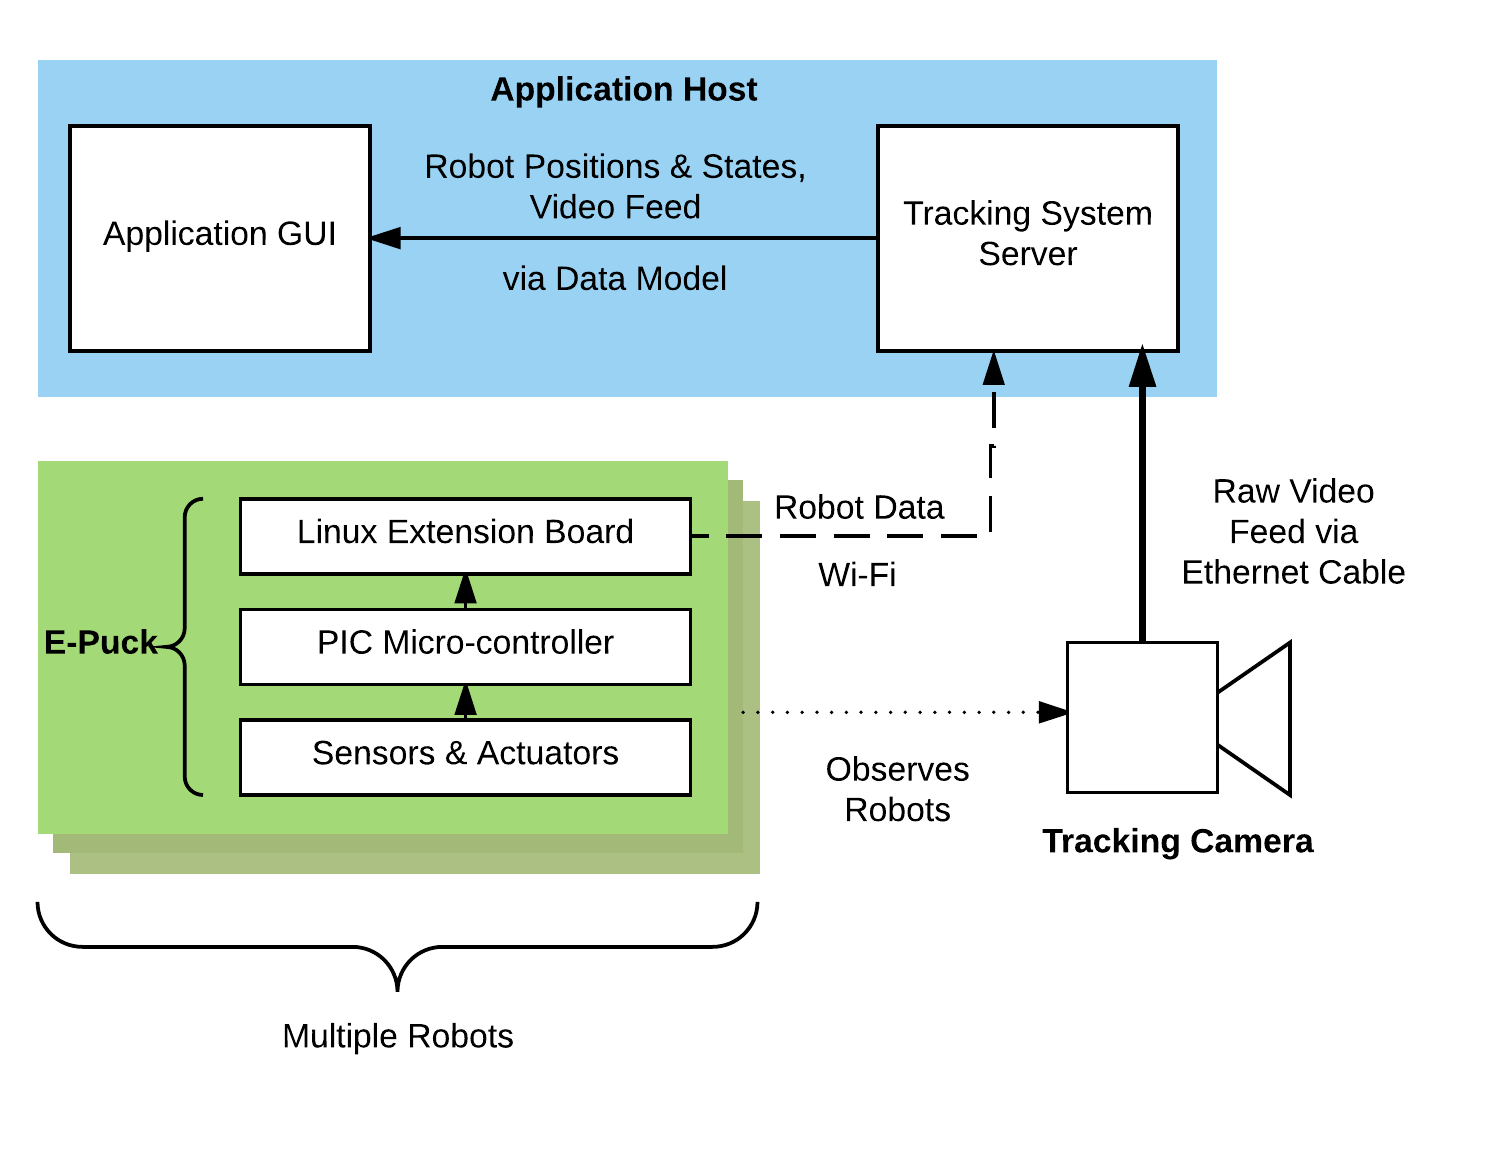
\includegraphics[scale=0.9]{SystemArchitecture.png}
	\caption{Expected general system architecture}
	\label{fig:SystemArchitecture}
	\end{center}
\end{figure}

\begin{multicols*}{2}

In order to be useful in swarm robotics experiments the system must be able to collate data on multiple active robots. The user must then be able to configure the data being displayed according to what is relevant for the current experiment. The user should also be able to access data related to a single robot at a time, as well as the swarm as a whole. The application will aim to make these configuration options available to the user through conventional application interface techniques.

\section{Specification}
Given the aims stated above, a specification for the system to be developed can be stated as follows. The system:

\begin{enumerate}
	\item Must be comprised of a PC application.
	\item Must receive data related to the state of multiple robots.
	\item Must receive positional data for the same set of robots.
	\item Must receive a live video feed of the robots in their environment.
	\item Must collate this data and present it to the user in a combined graphical form.
	\item Must present auxiliary, non-spatial data to the user in textual or other forms.
	\item Must update in approximately real time.
	\item Must at minimum support the E-Puck swarm robotics platform.
	\item Should use a modularised structure.
	\item Should exchange data between modules using a platform-agnostic, extensible protocol.
	\item Should provide a basis for interoperability with a number of robotics platforms.
	\item Should allow the user to configure the displayed data.
\end{enumerate}

\section{Literature Survey}
A number of key areas of literature have been identified as relevant to this project. A small body of work exists describing similar real time, graphical debugging systems for swarm and other robotics applications. These are primarily bespoke systems targeting single robotics platforms. These are considered in Section \ref{SimilarWork}. Some of the key works on swarm intelligence and swarm robotics as a whole are are highlighted in Section \ref{GeneralSR}, as an understanding of the fundamental concepts will be key to producing a useful application.  More specific work relating to human-swarm interaction and improvements to human-robot interaction through augmented reality (AR) tools are also considered, in section \ref{HumanSwarmInteraction}.

\subsection{Swarm Intelligence and Robotics Overview} \label{GeneralSR}
In his paper `\textit{Swarm Robotics: From Sources of Inspiration to Domains of Application}' Erol Sahin presents a summary of the key concepts of swarm robotics\cite{InspirationToApplication}, and attempts to offer a coherent definition of the topic. Sahin notes that a key difference from other multi-robot systems is the lack of centralised control, and the idea that behaviour should emerge from simple local interactions between robots, and between the robots and their environment. He also notes some of the key motivators behind Swarm Robotics research, noting that a swarm robotics system would ideally have `robustness', `flexibility' and `scalability'. Robustness refers to the swarms ability to continue to function should one or more individual swarm members suffer a failure of some kind. Flexibility refers to the swarm's ability to adapt to changes in the environment without the need for re-programming. Scalability describes the idea that a swarm should be functional at a range of sizes, and that ideally the number of robots in the swarm could be increased or decreased depending on the demands of the task. This idea of increasing a group size to tackle a specific task is sometimes referred to as 'recruiting'\cite{Recruiting}. Sahin also goes on to describe several classes of application area where Swarm Robotics systems might be well suited. !! In his paper `\textit{From Swarm Intelligence to Swarm Robotics}' Gerardo Beni presents a relatively informal overview of 

\subsection{Similar Work} \label{SimilarWork}
In their paper `Interactive Augmented Reality for Understanding and Analysing Multi-Robot Systems' Ghiringhelli et al. present a system for augmenting a video feed of an environment containing a number of robots with live information relating to each of the robots\cite{LEDSwarmAR}. The work presented mirrors closely the aims of this project. The authors identify the ability to overlay on to the video feed spatial information exposed by the robots, in the form of graphical representations situated relative to the tracked position of the related robot, as the most important debugging feature of the system. Each robot features a coloured LED blinking a unique coded pattern to enable tracking, and the system uses homography techniques to map between the robots' frame of reference and the camera's. This project intends to use a simpler approach, with position and orientation tracking achieved through the use of the AruCo marker-based tracking system, and a birds-eye view position for the camera to simplify mapping.

\subsection{Human-Swarm and Human-Robot Interaction} \label{HumanSwarmInteraction}


\section{Project Plan}
\begin{thebibliography}{1}
\bibitem{SwarmRoboticsDefinition} Swarm Robotics: From Sources of
Inspiration to Domains of Application, E. Sahin, 2005
\bibitem{SwarmIntelligence} Swarm intelligence. Dorigo M. Birattari M.
\bibitem{InspirationToApplication} E. S¸ahin and W.M. Spears (Eds.): Swarm Robotics WS 2004, LNCS 3342, pp. 10–20, 2005. Springer-Verlag Berlin Heidelberg 2005
\bibitem{FromSIToSR} E. S¸ahin and W.M. Spears (Eds.): Swarm Robotics WS 2004, LNCS 3342, pp. 1–9, 2005. Springer-Verlag Berlin Heidelberg 2005
\bibitem{LEDSwarmAR} Interactive Augmented Reality for Understanding and Analyzing Multi-Robot Systems Fabrizio Ghiringhelli
\end{thebibliography}

\end{multicols*}

\end{document}
